%TO-DO
%
% add figures, both for normal cases and for specific metrics
% [ IV in CBC vs CFB ]
% review pls!

\documentclass[11 pt]{article}
\usepackage{graphicx}
\title{
	The usage and the impact of shift registers on CFB \\
	\large HW1 - CNS Sapienza}

\author{Luigi Russo 1699981}
\date{12/10/2018}

\begin{document}

\maketitle



\section{Modes of operations}
Over the past years there has been a big effort in order to develop cryptographically strong algorithms, able to provide data confidentiality: and algorithms such as Rijndael, TwoFish, Serpent and RC6 have been produced, deeply analyzed and deployed. However, most algorithms accept a fixed-size input (e.g. 64 bits). Can this be considered a limit? Or, to be more precise, can this constraint limit the strength of such good algorithms? The truth is that it depends on how we handle the very common case of relatively long inputs: these handlers are also known as modes of operations; to be more formal, we could say that a block cipher mode of operation is a deterministic procedure (i.e. an algorithm itself) or a sequence of instructions and operations that have to be performed iteratively and applied to the original plaintext.
There is not a perfect mode of operation, in the sense that it depends on the application and the system requirements. Some of the most common modes are ECB, CBC, CFB, and OFB. Each of this has its own pros and cons; in next sections CFB mode is described.

\section{Overview of the CFB}
As said in the previous section, the Cipher Feedback Block (CFB) is a very common mode of operation. We first encrypt the initialization vector (IV). Once the encryption of a block has been computed, the result is XOR-ed with the corresponding plaintext block. We can note that the CFB is a particular stream-cipher, where the key scheduling depends on the IV and the algorithm used in each box. The IV does not need to be private, but it must be unpredictable, i.e. the attacker should not be able to know in advance the IV.
\begin{figure}[!ht]
	\centering % optional
	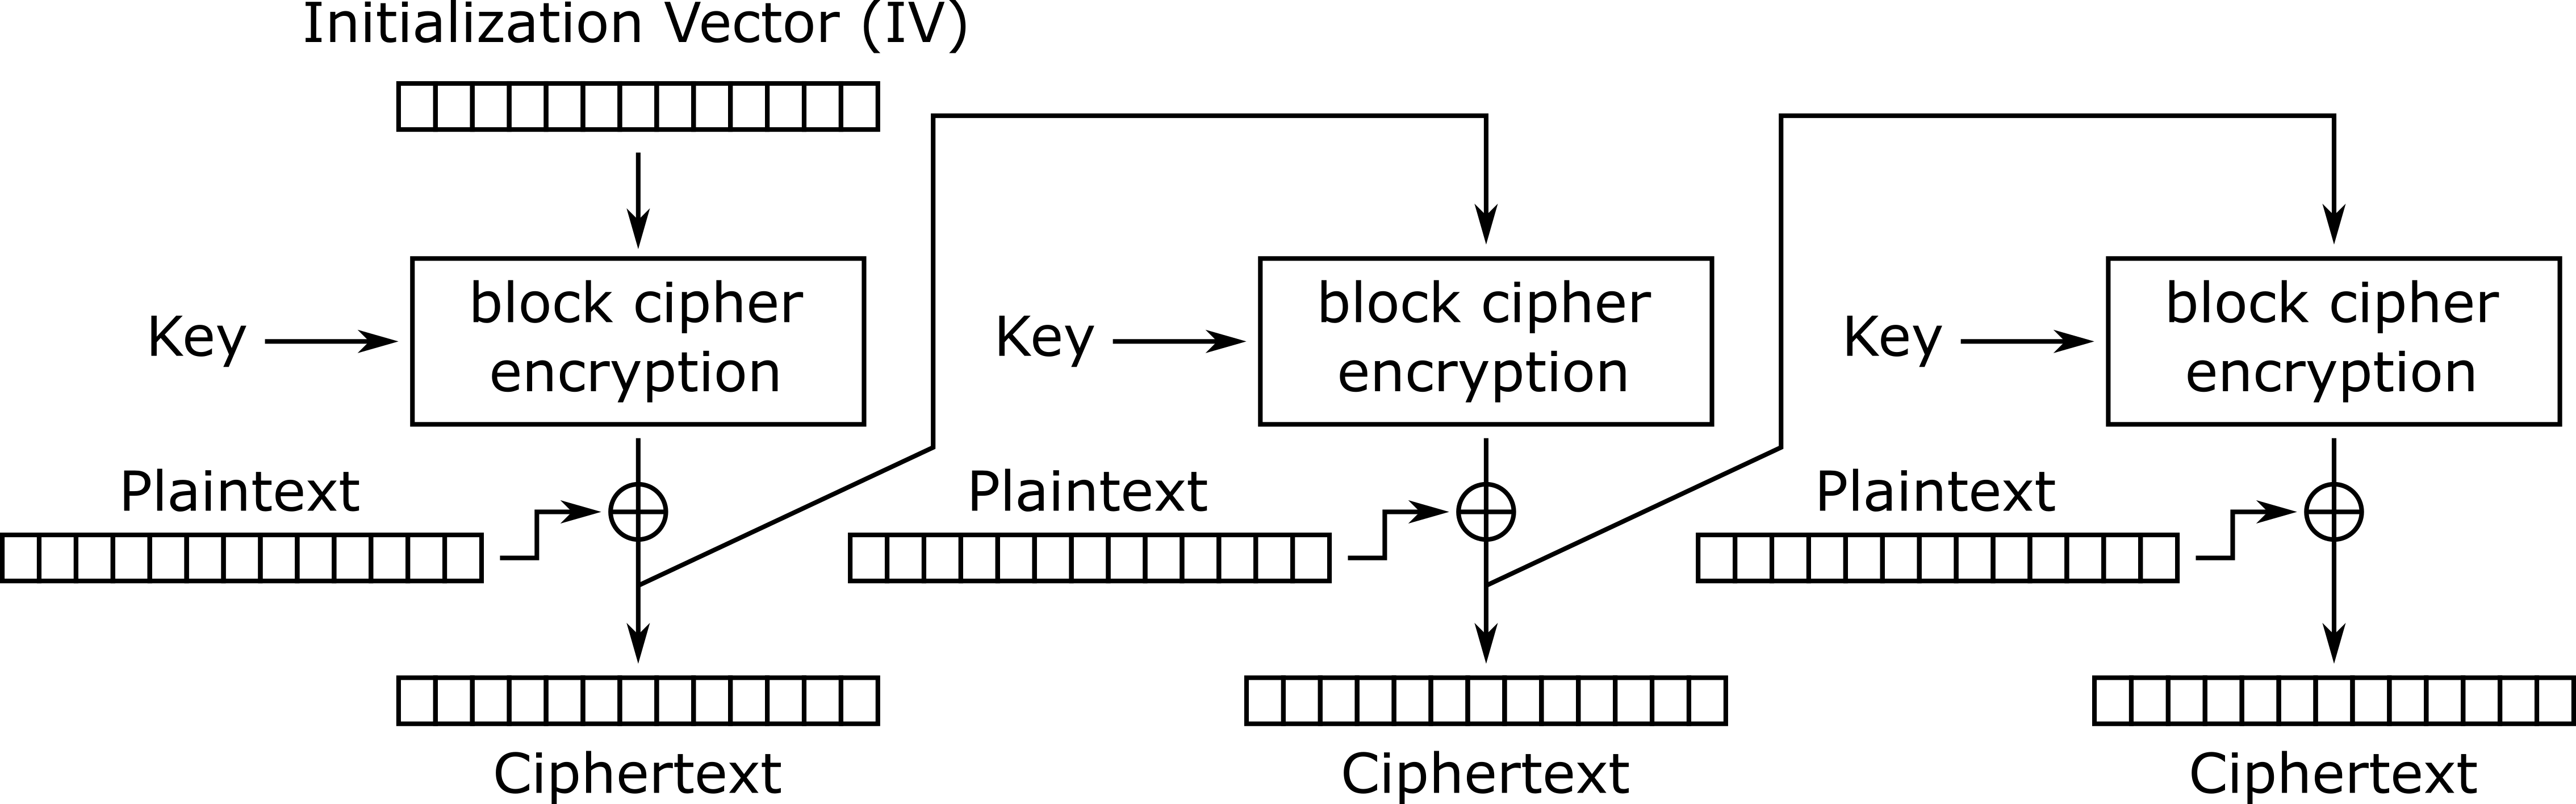
\includegraphics[width=1\textwidth]{CFB_encryption-hw1-1699981.png} % adjust width
	\caption{CFB encryption (from Wikimedia Commons)} % optional
	\label{fig:CFB_encryption}
\end{figure}
To decrypt the ciphertext, it is actually used the encryption algorithm: so, first of all the IV is encrypted and its output is XOR-ed with the first block of ciphertext, thus producing the first block of plaintext. Then, the first ciphertext is used for the next round and, again, the result is XOR-ed with second block of ciphertext, producing the second block of plaintext.
\begin{math}
\newline\newline
C_{0}= {\mbox{IV}}
\newline\newline
C_{i}=E_{K}(C_{i-1})\oplus P_{i}
\newline\newline
{P_{i}=E_{K}(C_{i-1})\oplus C_{i}}
\newline\newline
\end{math}
where $C_{i}$ is the i-th block of the ciphertext and $P_{i}$ is the i-th block of the plaintext; $ E_k $ is the encyption function used in each block and depends on the secret key K.
There are some aspects of this mode that have to be deepened in order to know what are its pros, its cons and the possible improvements.
\subsection{Performance metrics}
\subsubsection{Running in parallel}
The encryption phase cannot be run in parallel: in fact, we know that each block of the original text has to be encrypted dependently on previous ciphertext blocks: i.e. the encryption has to be performed in sequential way.
As for the decryption, instead, it can be performed in parallel; in particular, each plaintext block needs a pair of ciphertext blocks to be computed: as for the first block, we only need the first ciphertext block, since the IV is known by the decrypter.
\subsubsection{Chaining dependencies}
If the attacker is able to swap ciphertext blocks, the decrypter is not able to completely reconstruct the original message: in particular, we need \textbf{two correct blocks in a row} to successfully decrypt a plaintext segment.
\subsubsection{Error propagation}
If there is a single-bit error in a ciphertext block, we have a single-bit error in the corresponding plaintext block and the next one is completely lost, because of the strength and the non-linearity of the encryption function. It is important to note that an adversary may cause predictable bit changes in a plaintext segment, simply modifying the corresponding bits of the ciphertext.
\subsubsection{Error recovery}
If any  bit is lost (or added) in a block (we call this kind of error a \textit{slip}) it is not possible to re-synchronize and eventually decrypt successfully the next blocks. So the CFB is really weak against attacks where bits are added to or removed from the message.
\subsubsection{Throughput}
The CFB needs the last block to be padded if the total length of the plaintext is not a multiple of the ciphertext block-size. However, we also know that ciphertext stealing is a valid approach to not pad the message with bits; moreover, padding a message is a very simple strategy to avoid that even its length is disclosed to the attacker, so in most cases it is still recommended to adopt it.
\subsubsection{Random read access}
The CFB supports the random read access, meaning that we can decrypt a segment of ciphertext in arbitrary position: it is obvious that to \textit{read} the segment $P_i$ we only need the two consecutive ciphertext blocks $C_i$ and $C_{i-1}$.
\subsection{Other considerations}
Since both encryption and decryption use the same encryption function, the CFB can be used if and only if the block cipher uses a private-key algorithm. Moreover, the IV should not be reused to encrypt future messages.
\subsection{Can we do better than the CFB?}
We could finally summarize the main weaknesses of this mode:
\begin{enumerate}
	\item It is not efficient to send very short messages (e.g. send 1 byte when block-size is 4 bytes).
	\item It is not self-synchronizing, meaning that if some bits are added or lost the plaintext cannot be reconstructed.
	\item Allows the attacker to cause predictable bit changes in a plaintext segment.
	\item No real advantage to use it instead of the CBC mode. \cite{Crypto Book}
\end{enumerate}
A nice workaround to (1) and, under some restrictions, to (2) and (4), consists of using shift registers.  
\section{The CFB with shift registers}
Given the IV, it is encrypted and the first output block is produced. This is not the first ciphertext block at all. In order to produce that, we compute the XOR between the first plaintext segment and the \textit{s} most significant bits of the first output block. For the second block to be encrypted, we still need a block of size \textit{n}: so we use the \textit{n-s} least significant bits of the IV and concatenate them with the \textit{s} bits of the first ciphertext segment to form the second input block. After some rounds, the IV is completely replaced by ciphertext bits. The precise number of rounds after which the IV is replaced (and more in general, after which the contribute of a ciphertext block to the next encryptions ends) depends of course on the number \textit{s} of bits that shift at each round and on the number \textit{n} that is the size of the block: it is equal, of course, to \textit{n/s}.
\begin{figure}[!ht]
	\centering % optional
	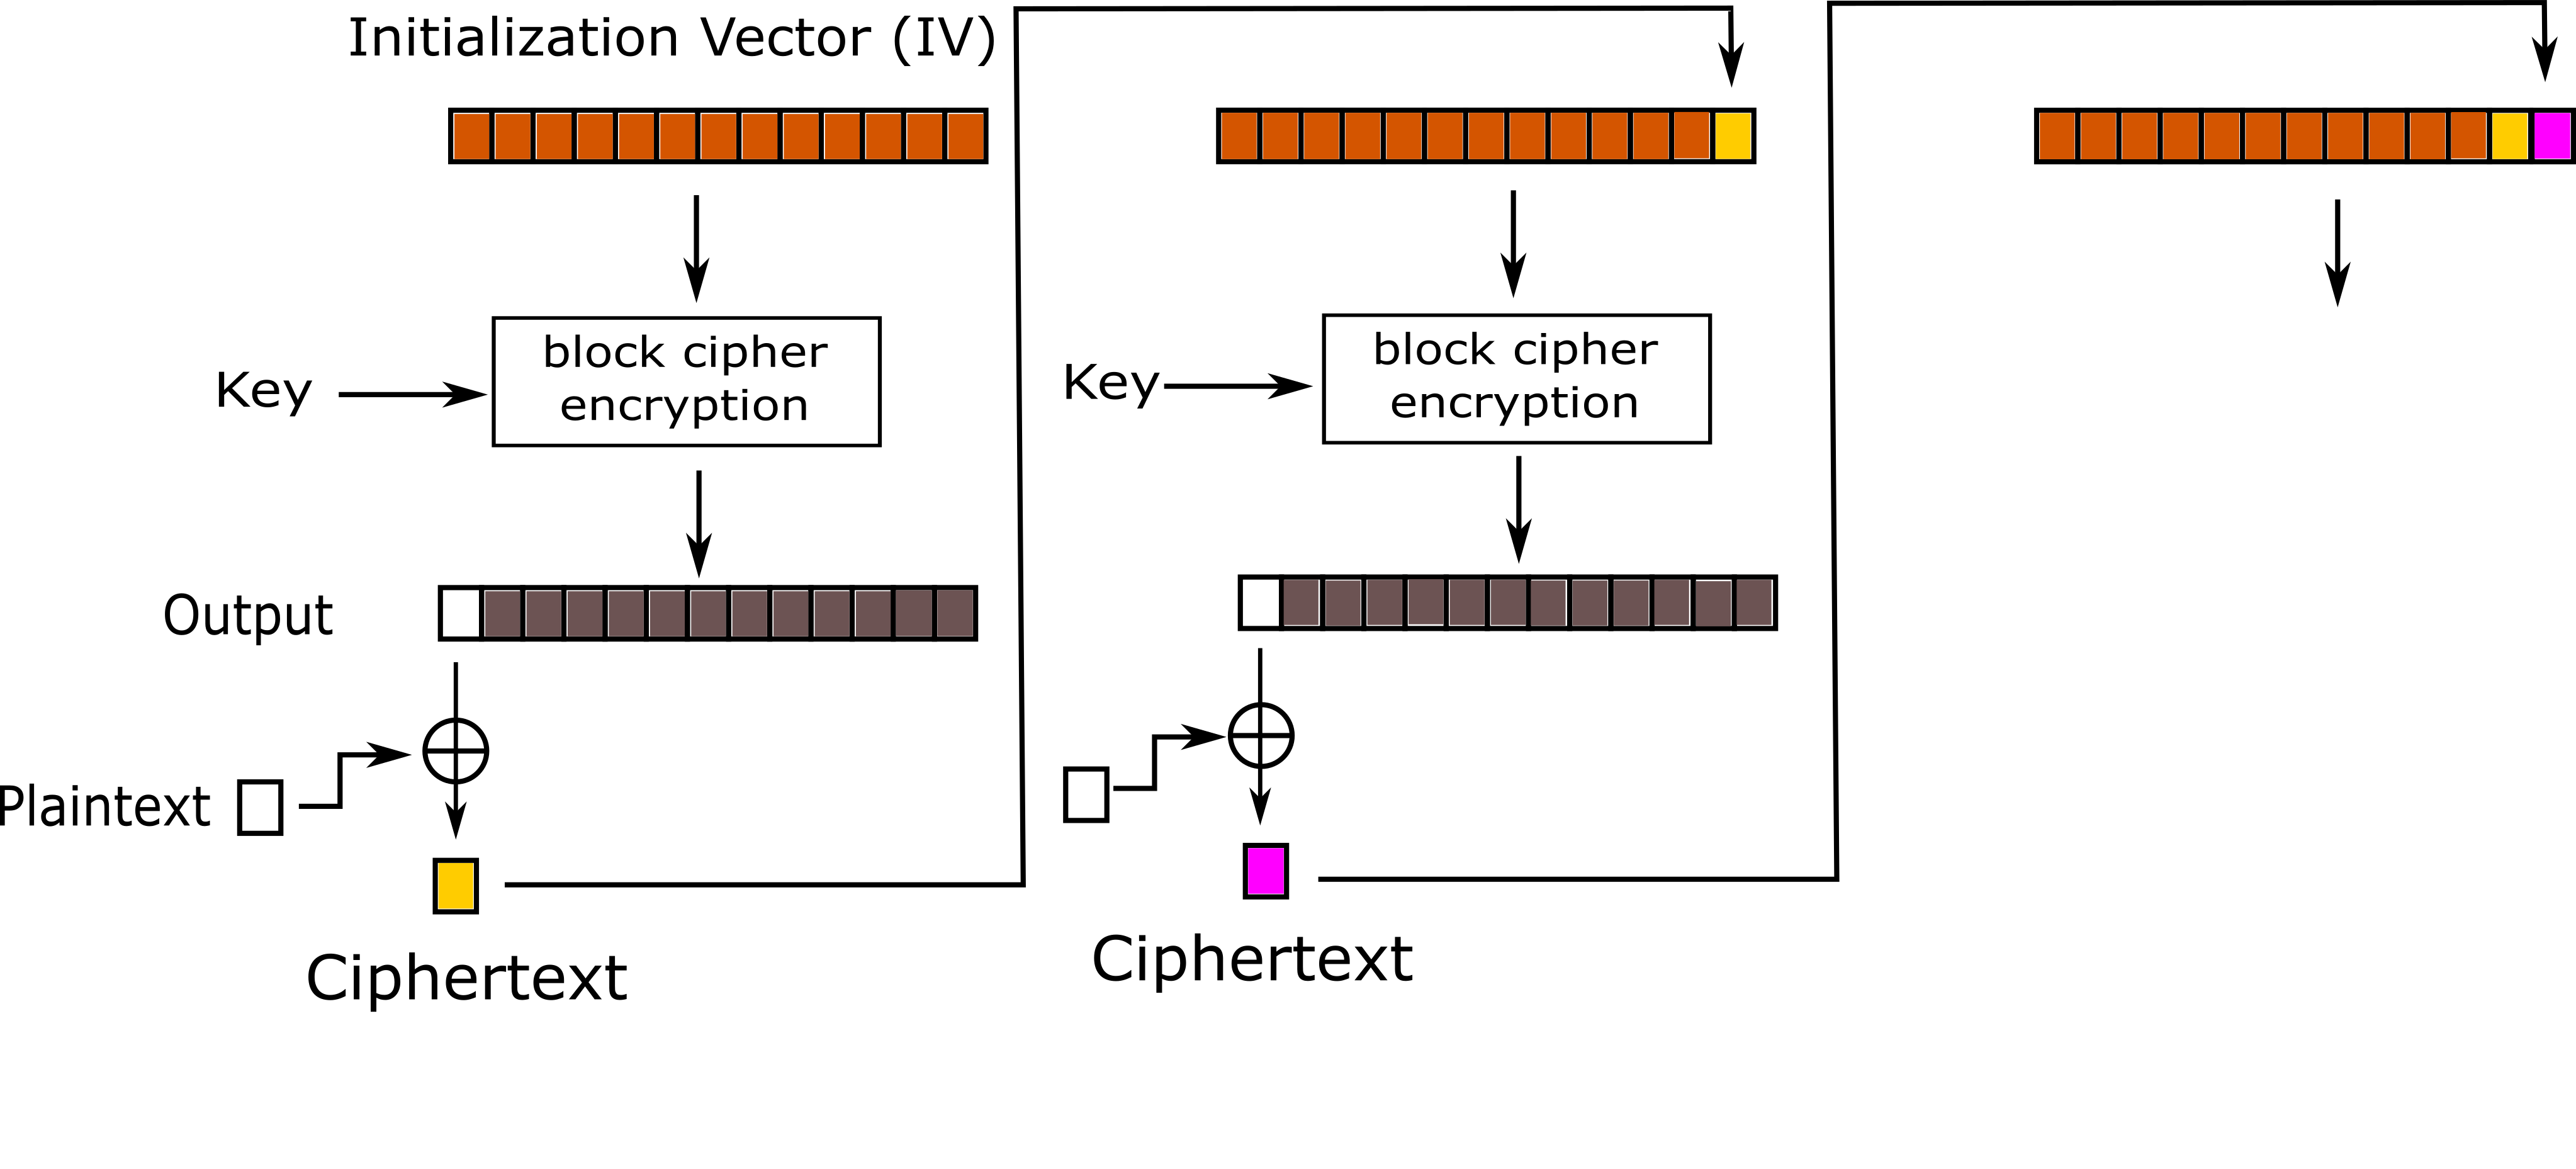
\includegraphics[width=1\textwidth]{1_CFB_encryption-hw1-1699981.png} % adjust width
	\caption{1-CFB encryption} % optional
	\label{fig:1_CFB_encryption}
\end{figure}

In more formal way, if we define $ S_i $ as the i-th state of the shift register, a $<<$ x as a shifted up x bits, $MSB_x(a)$ as the x most significant bits of a, and n as the number of bits of IV, we have:
\begin{math}
\newline\newline
S_{0}= {\mbox{IV}}
\newline\newline
S_{i} = ((S_{i-1}<<s)+C_{i}){\mbox{ mod }}2^{n}
\newline\newline
C_{i}={\mbox{MSB}}_s(E_{K}(S_{i-1}))\oplus P_{i}
\newline\newline
\end{math}
The decryption is quite the same: the IV is still the first input block, while the next input blocks are produced by concatenating the \textit{n-s} least significant bits of the previous input block with the \textit{s} most significant bits of the previous ciphertext block. Each input block is then encrypted and an output block is produced. Its \textit{s} most significant bits are XOR-ed with the corresponding ciphertext blocks in order to obtain the plaintext.

$ \newline P_{i}={\mbox{MSB}}_s(E_{K}(S_{i-1}))\oplus C_{i} \newline $

\subsection{Performance metrics}
\subsubsection{Running in parallel}
As for the parallelization, there is no difference with the respect to the pure CFB mode: so, decryption is parallelizable, while encryption is not.
\subsubsection{Chaining dependencies}
Again, if the attacker is able to swap ciphertext blocks, the decrypter is not able to completely reconstruct the original message. In order to correctly decrypt a plaintext segment we need in particular \textbf{n/s correct blocks in a row}, where \textit{s} is both the size of each plaintext segment and the number of bits shifted at each round.
\subsubsection{Error propagation}
The fact that a single-bit error in a ciphertext block causes a single-bit error in the corresponding plaintext block is still true: an adversary may cause predictable bit changes in a plaintext segment. Moreover, when a single-bit (or few bits) error occurs in a block, we cannot correctly decrypt the next \textit{n/s} ciphertext blocks, as they depend on the previous corrupted one.
\begin{figure}[!ht]
	\centering % optional
	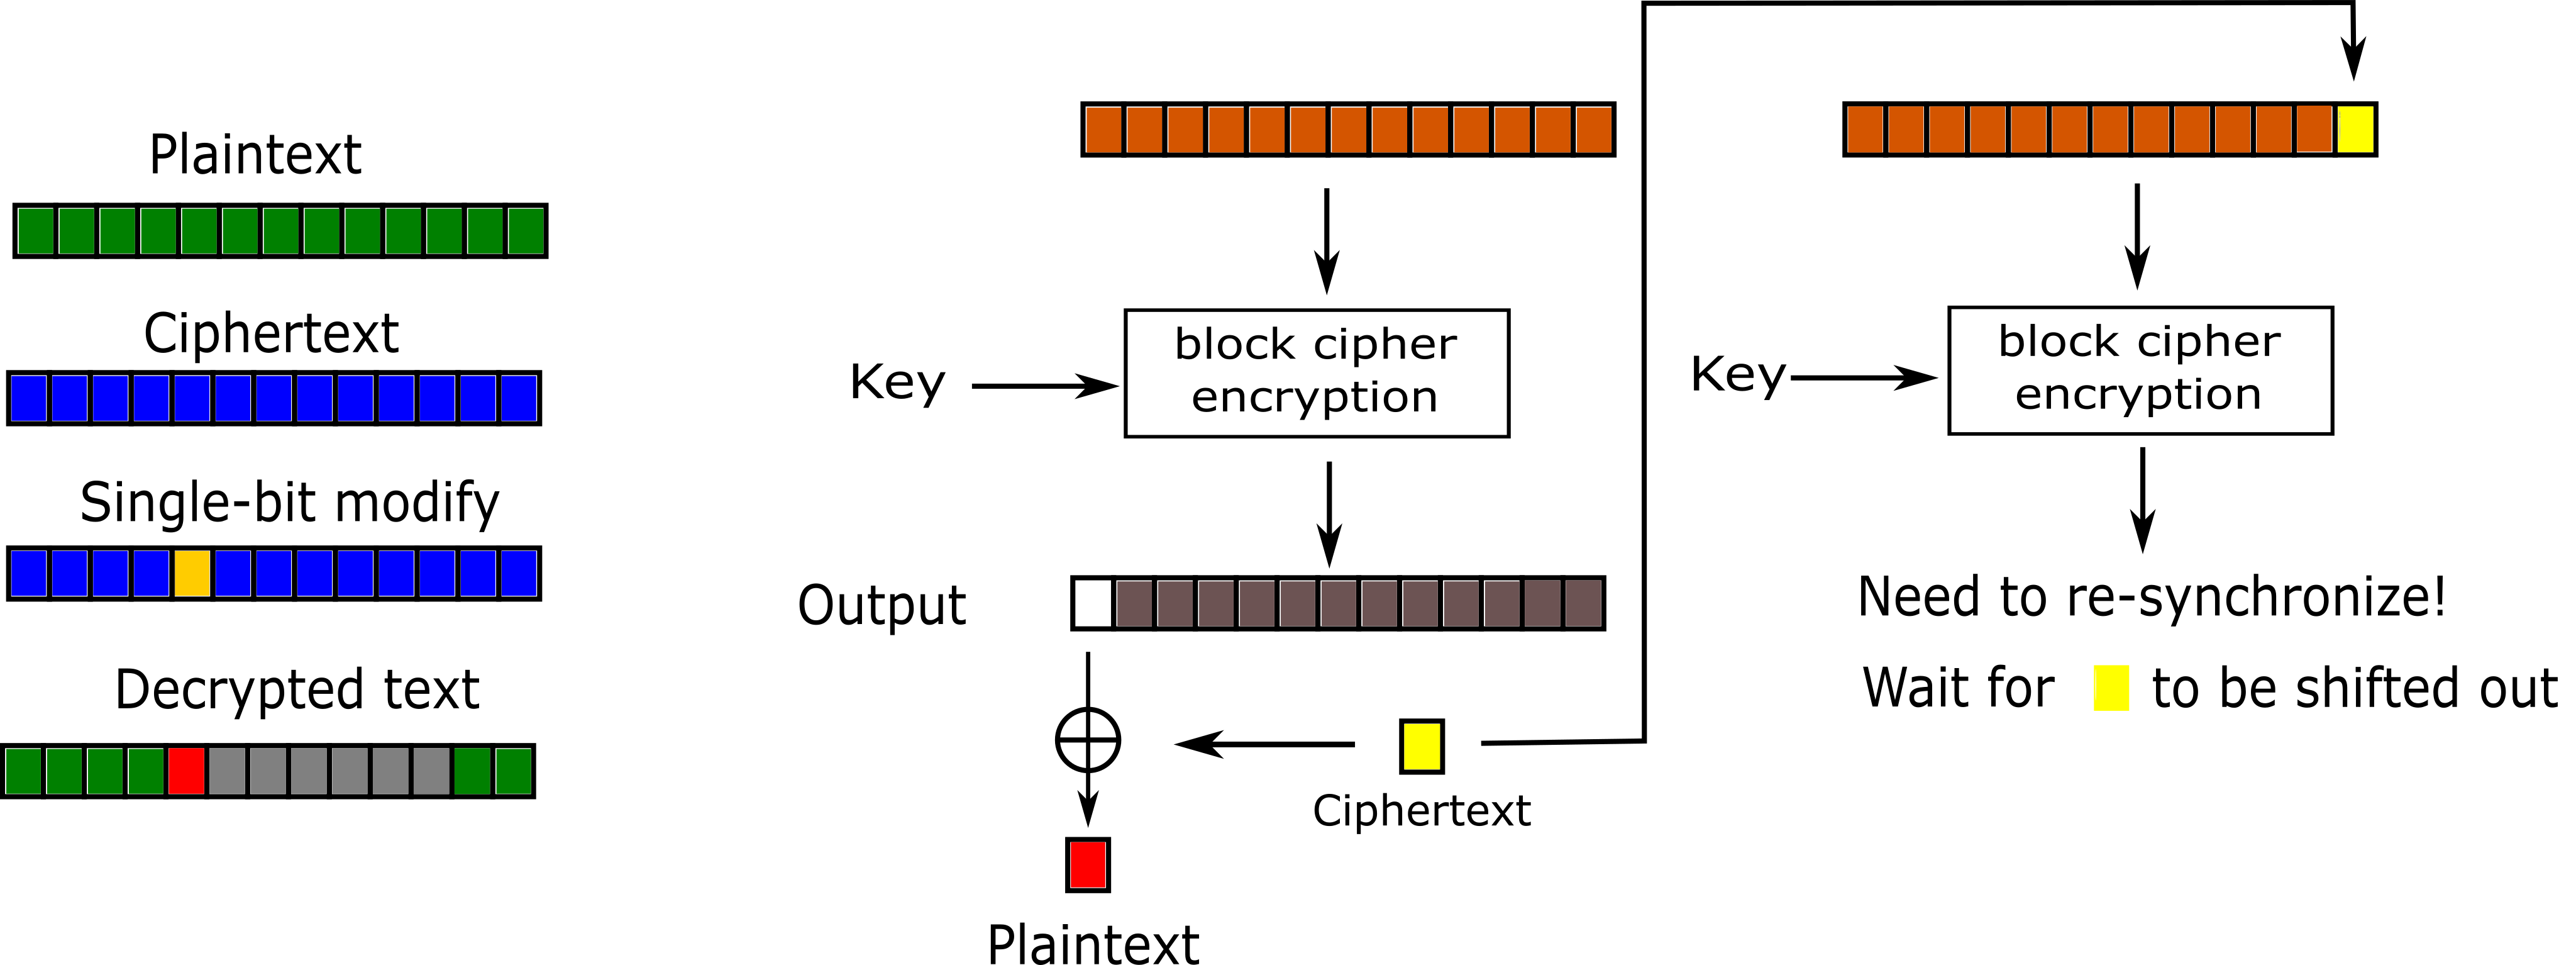
\includegraphics[width=1\textwidth]{1_CFB_single_bit_error-hw1-1699981.png} % adjust width
	\caption{1-CFB, single-bit error producing predictable change in plaintext and re-synchronization} % optional
	\label{fig:1_CFB_single_bit_error}
\end{figure}
\subsubsection{Error recovery}
When an entire block is lost, this mode provides self-synchronization, as the CBC. But \textit{n/s} blocks are required (meaning that have to skipped) in order to recover the error and re-synchronize with the sender.
What happens if a number \textit{k} less than the block-size is lost? It depends on the number \textit{s} of shifted bits. So, if \textit{k} is a multiple of \textit{s}, after some blocks (again, these have to be "skipped") we finally re-synchronize. If \textit{s} is 1, it is always possible to recover the \textit{slip} and restore the synchronization \textit{n + 1} bits after the deleted (or added) bit \cite{NIST mop}. But, in general, due to efficiency issues, it is preferable to use \textit{s} equal to 8 or multiple of 8, so that we can recover if and only if multiple of bytes are lost (or added by the attacker).
\subsubsection{Throughput}
This mode does not need the message to be padded; and this is a very nice feature, especially if we need to stream messages or the size of our messages is often very short (i.e. few bits). 
We have to note that if \textit{s} less than \textit{n}, then the throughput is decreased by a factor of \textit{n/s} \cite{Crypto Book}, meaning that each round of encryption is actually encrypting (processing) \textit{s} bits of the plaintext. And this really limits the throughput of this mode \cite{Performance comparison}; for this reason, \textit{s} = 8, 64, 128 are preferable to \textit{s} = 1, although they are weaker to error recovery, as stated in the previous section. %We must finally note that the encryption function should not be very "" since it has to be computed more times. 
\subsubsection{Random read access}
It also supports the random read access: to \textit{read} the segment $P_i$ we need at most\footnote{We cannot use the adverb \textbf{exactly} because the precise number of blocks depends on the position of the block we want to \textit{randomly} access. For instance, the second block needs only the two previous blocks to be successfully decrypted; however, we can fix the upper-bound to \textit{n/s}, because when the contribute of the IV is over, \textit{n/s} is the true number of consecutive blocks we actually need for a random read access.} \textit{n/s} consecutive ciphertext blocks.
\subsection{Other considerations}
The considerations about public-key algorithms still remain true, so only private-key algorithms can be used in the blocks of the CFB.

% put after conclusion
\begin{thebibliography}{10}

	% bibitem for paper
	\bibitem{NIST mop}
	Morris Dworkin, ``Recommendation for Block Cipher Modes of Operation,'' {\em NIST Special Publication 800-38A},
	2001.
	
	\bibitem{Crypto Book}
	A. J. Menezes, P. C. van Oorschot, S. A. Vanstone, ``Handbook of Applied Cryptography''
	
	\bibitem{Performance comparison}
	M. Alfadel, E. M. El-Alfy, K. Kamal, ``Evaluating time and throughput at different modes of operation in AES algorithm''
	
	
\end{thebibliography}

\end{document}
